% =============================================================================
% 中国科学院大学《计算机体系结构（研讨课）》实验报告 LaTeX 模版（单文件版）
% 版本：v1.0  日期：2026-09
% 参照《计算机组成原理（研讨课）》实验报告模版（ucas_cod_lab_report_v10，
% 由 Shing-Ho Lin、Jun-Xiong Ji 编写）改写，仅供课程实验报告排版使用。
%
% 【编译方式】
%   使用 XeLaTeX 编译（需 TeX Live 2023 及以上，含 ctex 宏集）：
%     xelatex tamplate.tex      % 连续编译两次，以正确生成交叉引用与页码
%   或： latexmk -xelatex tamplate.tex
%
% 【字体与排版】
%   正文 11pt，A4 纸，页边距左右 2.0cm、上下 2.5cm；
%   中文使用 ctex 默认系统字体（Windows 下为宋体正文、黑体标题、楷体强调 \kaishu），
%   不依赖外部字体文件，模版可单独拷贝使用；标点采用开明风格；
%   章节序号为中文「一、二、…」，小节序号为阿拉伯数字；页脚居中显示页码。
%
% 【主要宏包】
%   ctex（中文排版）、geometry（页面设置）、graphicx/subfigure（插图与并排图）、
%   amsmath 等（数学公式）、listings（代码）、booktabs/tabularx/multirow/bigstrut
%   （表格）、float（[H] 浮动体定位）、tikz/xcolor（绘图与颜色）、zhnumber（中文
%   序号）、cleveref（\cref 交叉引用）、fancyhdr（页眉页脚）、algorithm 系列
%   （算法伪代码）、mdframed（带边框文本块）等，详见下方导言区。
%
% 【使用方法】
%   1. 修改下方 \name、\studentNum、\major、\labNum、\labName 表头宏为真实信息；
%   2. 将 draw.io、Visio 等导出的 PDF 图片放入 fig/ 目录后插入；fig/ 中现有
%      两张示例图片仅供编译演示，可直接替换或删除；
%   3. 按各章节的占位说明填写内容，删除占位文字与用法示例即可；
%   4. 报告不加目录；全文的标题、正文、图表标题与表中内容格式应保持统一；
%   5. 本模版仅提供报告结构与排版参考，可包含但不限定其中的条目；报告中
%      无需重复描述讲义中的实验流程；图表请尽量使用 draw.io、Visio 等作
%      图软件绘制后插入。
%
% 【模版结构】
%   一、设计思路（总体结构、关键设计及巧妙之处、设计难点）
%   二、实现与结果（关键代码、测试方法与实验结果）
%   三、调试与问题定位（问题总结表、高质量 bug 定位过程）
%   四、总结与思考（收获与不足）
%   五、实验时长
% =============================================================================

\documentclass[11pt]{article}

\usepackage[a4paper]{geometry}
\geometry{left=2.0cm,right=2.0cm,top=2.5cm,bottom=2.5cm}

\usepackage{ctex} % 支持中文的LaTeX宏包
\usepackage{amsmath,amsfonts,graphicx,subfigure,amssymb,bm,amsthm,mathrsfs,mathtools,breqn} % 数学公式和符号的宏包集合
\usepackage{algorithm,algorithmicx} % 算法和伪代码
\usepackage[noend]{algpseudocode} % 算法和伪代码
\usepackage{fancyhdr} % 自定义页眉页脚
\usepackage[framemethod=TikZ]{mdframed} % 创建带边框的框架
\usepackage{fontspec} % 字体设置
\usepackage{adjustbox} % 调整盒子大小
\usepackage{fontsize} % 设置字体大小
\usepackage{tikz,xcolor} % 绘制图形和使用颜色
\usepackage{multicol} % 多栏排版
\usepackage{multirow} % 表格中合并单元格
\usepackage{pdfpages} % 插入PDF文件
\usepackage{listings} % 在文档中插入源代码
\usepackage{wrapfig} % 文字绕排图片
\usepackage{bigstrut,multirow,rotating} % 支持在表格中使用特殊命令
\usepackage{booktabs} % 创建美观的表格
\usepackage{circuitikz} % 绘制电路图
\usepackage{zhnumber} % 中文序号（用于标题）
\usepackage{tabularx} % 表格折行
\usepackage{float} % 支持 [H] 浮动体定位

\definecolor{dkgreen}{rgb}{0,0.6,0}
\definecolor{gray}{rgb}{0.5,0.5,0.5}
\definecolor{mauve}{rgb}{0.58,0,0.82}
\lstset{
  frame=tb,
  aboveskip=3mm,
  belowskip=3mm,
  showstringspaces=false,
  columns=flexible,
  framerule=1pt,
  rulecolor=\color{gray!35},
  backgroundcolor=\color{gray!5},
  basicstyle={\small\ttfamily},
  numbers=none,
  numberstyle=\tiny\color{gray},
  keywordstyle=\color{blue},
  commentstyle=\color{dkgreen},
  stringstyle=\color{mauve},
  breaklines=true,
  breakatwhitespace=true,
  tabsize=3,
}

% 轻松引用, 可以用\cref{}指令直接引用, 自动加前缀.
% 例: 图片label为fig:1
% \cref{fig:1} => 图 1
% \ref{fig:1}  => 1
\usepackage[capitalize]{cleveref}
\crefname{figure}{图}{图}
\crefname{table}{表}{表}
\crefname{equation}{式}{式}
\crefname{section}{节}{节}
\crefname{subsection}{节}{节}

% 若需使用自带字体文件，可取消以下注释，并将 font/ 目录下的 ttf 放在同级目录
% \setmainfont{Palatino Linotype.ttf}
% \setCJKmainfont{SimHei.ttf}
% \setCJKsansfont{Songti.ttf}
% \setCJKmonofont{SimSun.ttf}
\punctstyle{kaiming}

\renewcommand{\emph}[1]{\begin{kaishu}#1\end{kaishu}}

% 对 section 等环境的序号使用中文
\renewcommand \thesection{\zhnum{section}、}
\renewcommand \thesubsection{\arabic{subsection}}

% 页脚居中显示页码
\pagestyle{fancy}
\fancyhf{}
\fancyfoot[C]{\thepage}
\renewcommand{\headrulewidth}{0pt}

%%%%%%%%%%%%%%%%%%%%%%%%%%%
%改这里可以修改实验报告表头的信息
\newcommand{\name}{李四}
\newcommand{\studentNum}{2066K8009900000}
\newcommand{\major}{计算机科学与技术}
\newcommand{\labNum}{1}
\newcommand{\labName}{请按讲义填写实验名称}
%%%%%%%%%%%%%%%%%%%%%%%%%%%

\begin{document}

\begin{center}
  \LARGE \bf 中国科学院大学 \\《计算机体系结构（研讨课）》实验报告
\end{center}

\begin{center}
  \emph{姓名} \underline{\makebox[7em][c]{\name}} 
  % 如果名字比较长, 可以修改box的长度"7em"为其他值
  \emph{学号} \underline{\makebox[12em][c]{\studentNum}}
  \emph{专业} \underline{\makebox[15em][c]{\major}}\\
  \emph{实验项目编号} \underline{\makebox[3em][c]{\labNum}}
  \emph{实验名称} \underline{\makebox[30em][c]{\labName}}\\
\end{center}

\section{设计思路}

本部分应说明设计目标与总体方案，重点阐述设计思路、方案中的重点难点或自觉巧妙之处，并配以结构设计框图、状态转换图、流程图等说明，做到“一图胜千言”。

\subsection{设计目标与总体结构}

请在此处概述实验的设计目标、总体结构及模块划分，给出结构设计框图，并对图中各模块的功能与数据通路作简要说明。

\begin{figure}[htbp]
  \centering
  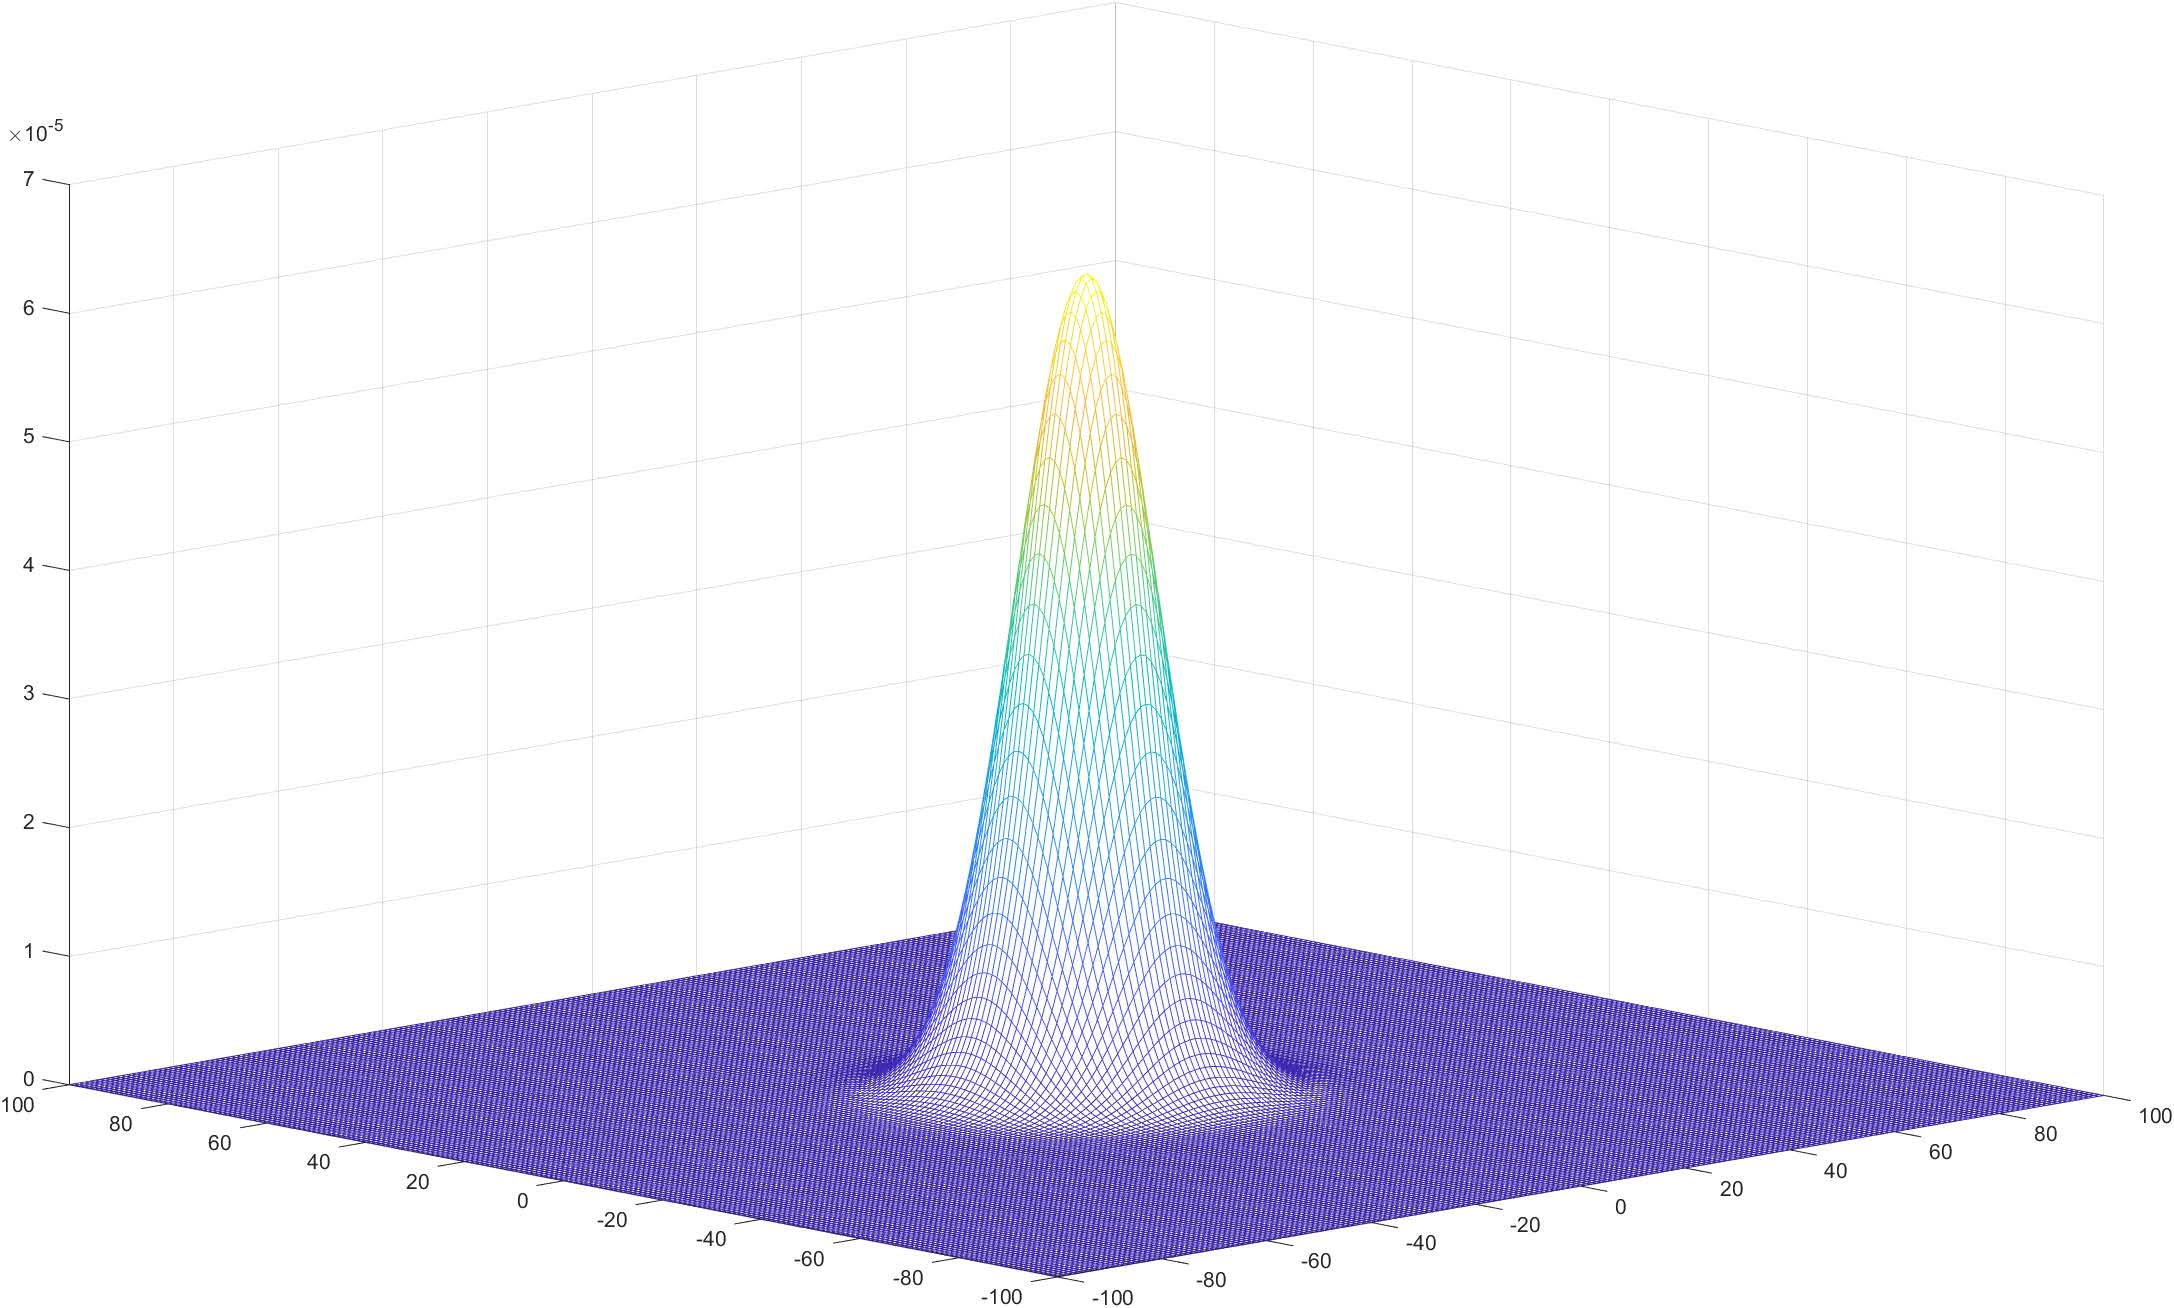
\includegraphics[width=10cm]{fig/Gaussian.pdf}
  \caption{设计总体结构框图（占位图，请替换为实际图片）}
  \label{fig:arch}
\end{figure}

如\cref{fig:arch}所示，本设计由……（此处为交叉引用示例：\verb|\cref{fig:arch}| 自动生成“图 1”）。

\subsection{关键设计与巧妙之处}

请在此处说明关键模块的设计方案与实现理由，例如流水线、Cache、分支预测、总线、特权级等设计；对自认为巧妙的设计处理应重点展开，必要时结合状态转换图、流程图或时序图说明。

\subsection{设计难点与解决方案}

请在此处列出设计中的重点与难点，说明所采用的解决方案及其取舍。

\section{实现与结果}

\subsection{关键实现与代码}

请结合设计思路对关键实现作简要说明，并附包含注释的关键代码段。代码不宜大段粘贴，只保留最能说明设计思想的部分。

\begin{lstlisting}[language=Verilog]
// 关键代码段示例（占位，请替换为实际代码）
module example (
    input  wire clk,
    input  wire rst_n,
    output reg  valid
);
    always @(posedge clk or negedge rst_n) begin
        if (!rst_n) valid <= 1'b0;
        else        valid <= 1'b1;
    end
endmodule
\end{lstlisting}

\subsection{测试方法与实验结果}

请说明验证方法（仿真激励、测试用例、FPGA 上板验证等）与实验所得结果，用图表给出关键数据或波形，并对结果作简要分析。

\begin{table}[htbp]
  \centering
  \begin{tabular}{c|c|c|c}
    测试用例 & 输入 & 预期结果 & 实际结果 \\
    \hline
       &      &      &      \\
    \hline
       &      &      &      \\
  \end{tabular}
  \caption{功能测试结果（占位表，请替换）}
  \label{tab:testresult}
\end{table}

\begin{figure}[H]
  \centering
  \subfigure[复位后波形]{
    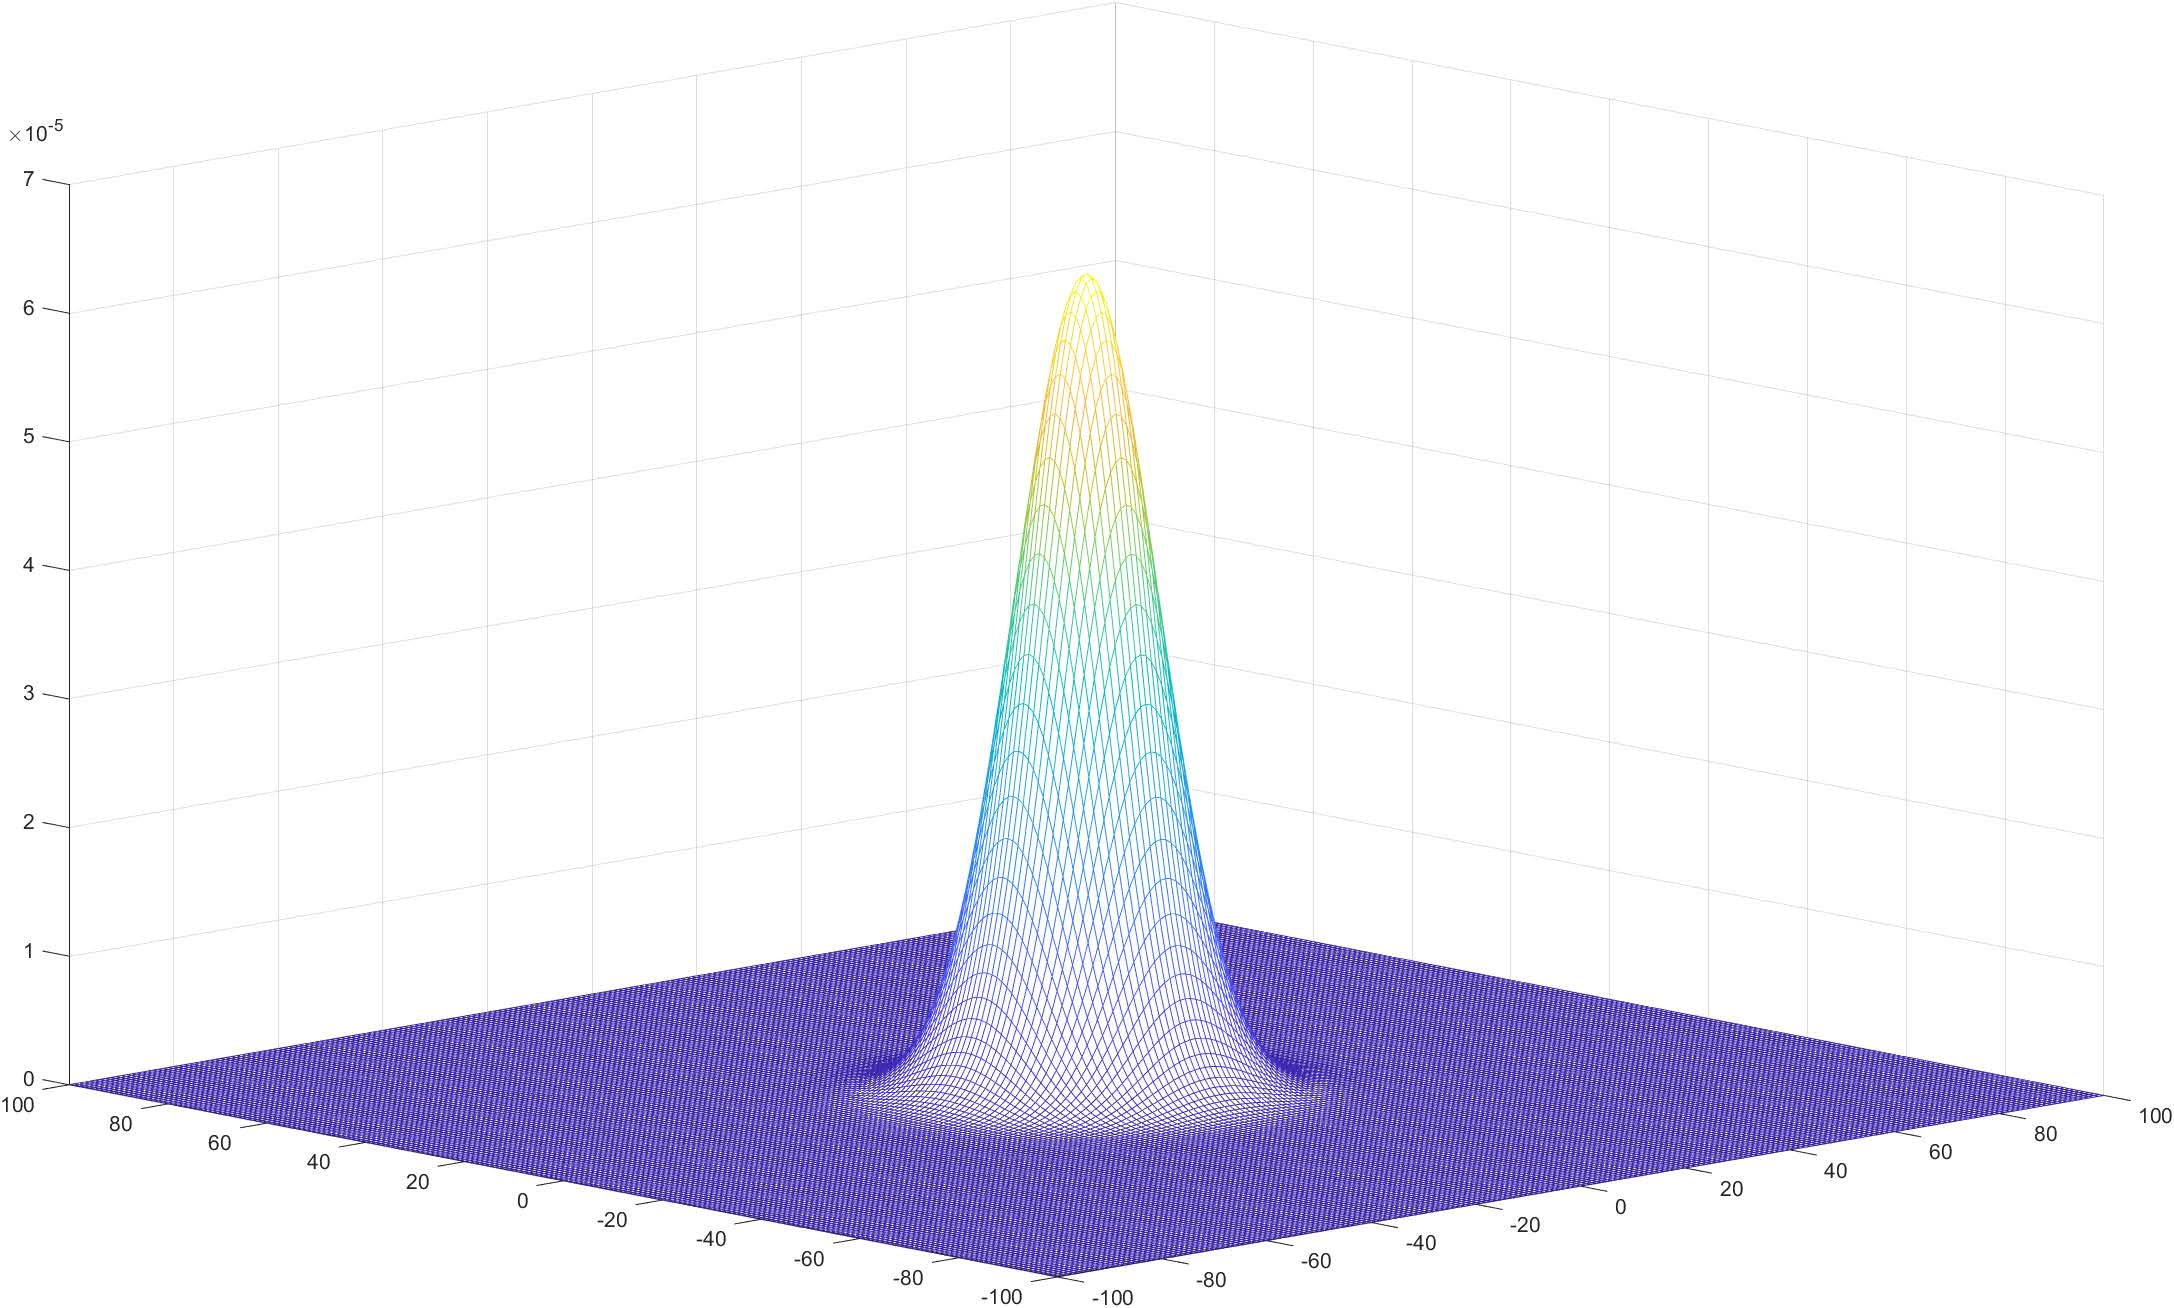
\includegraphics[width=7cm]{fig/Gaussian.pdf}}
  \hspace{0.3in}
  \subfigure[正常执行波形]{
    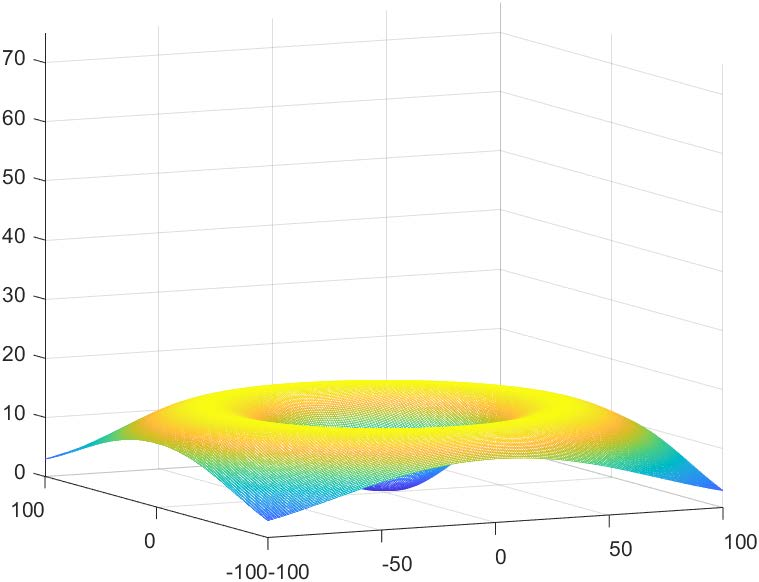
\includegraphics[width=7cm]{fig/Maxwell.pdf}}
  \caption{仿真波形对比（占位图，请替换为实际波形）}
  \label{fig:wave}
\end{figure}

\section{调试与问题定位}

本部分记录实验过程中遇到的问题及定位、解决过程，重点是“高质量”bug 的分析思路。出错模块指设计章节中列出的各个模块；问题类别包括逻辑电路设计、RTL 语法、行为仿真和逻辑综合等。

\begin{table}[htbp]
  \centering
  \begin{tabular}{c|c|c|c|c|c}
    序号 & 问题类别 & 出错模块 & 问题现象 & 产生原因 & 解决办法 \\
    \hline
       &      &      &      &      &      \\
    \hline
       &      &      &      &      &      \\
  \end{tabular}
  \caption{实验问题总结（占位表，请替换）}
  \label{tab:problem}
\end{table}

\noindent
$\bullet$
\textbf{高质量 bug 定位过程示例}：请选择调试过程中典型的一个问题，按“问题现象 $\rightarrow$ 假设与验证 $\rightarrow$ 根本原因 $\rightarrow$ 修复与验证”的思路完整记录定位过程，复杂问题可结合时序图说明。

\vspace{1ex}

\noindent
$\bullet$
\textbf{其他问题补充}：请编写你的实验报告内容。

\section{总结与思考}

\subsection{收获与不足}

请总结本次实验中的亮点与不足：亮点可说明后续补充计划，不足可说明后续提升计划；任务划分、联合调试等团队协作过程中的得失体会也可在此说明。

\section{实验时长}

\newcommand{\labTime}{123} % 请在这里填写实验所耗时间（单位：小时）

在课后，你花费了大约\underline{\makebox[5em][c]{\labTime}}小时完成此次实验，其中各个阶段的用时如\cref{tab:time_token}所示。

\begin{table}[htbp]
  \centering
  \begin{tabular}{c|c|c}
    步骤 & 时长（小时） & 说明 \\
    \hline
    设计 &        &    \\
    \hline
    开发 &        &    \\
    \hline
    调试 &        &    \\
  \end{tabular}
  \caption{实验时长}
  \label{tab:time_token}
\end{table}

\end{document}
